\section{Algorithm}

\begin{frame}
  \frametitle{Algorithm Outline}
  \begin{enumerate}
    \item Cost Graph Construction
    \item Forest Building
    \item Partition Refinement
  \end{enumerate}
\end{frame}

\begin{frame}
  \frametitle{Cost Graph Construction}
  \begin{columns}
    \column{.5\textwidth}
    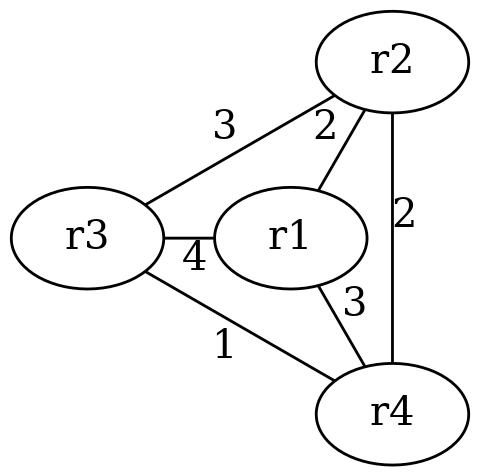
\includegraphics[width=140px]{../graphs/cost-graph.png}
    \column{.5\textwidth}
    \begin{block}{edge weight}
      \(w(e)=\sum_{j}^{} \frac{h_{a,b}(j)}{l_{j}}\) \\
      \scriptsize{
	\textcolor{red}{ \(h_{a,b}\) } generalization cost of items a and b \\
	\textcolor{red}{ \(l_{j}\) } maximum levels of generalization for column j
      }
    \end{block}
  \end{columns}
\end{frame}

\begin{frame}
  \frametitle{Forest Building}
  \begin{center}
    \begin{figure}[ht]
      \begin{overlayarea}{150px}{150px}
	\includegraphics<1>[width=140px]{../graphs/cost-graph-s0.png}
	\includegraphics<2>[width=140px]{../graphs/cost-graph-s1.png}
	\includegraphics<3>[width=140px]{../graphs/cost-graph-s2.png}
	\includegraphics<4>[width=140px]{../graphs/cost-graph-s3.png}
	\includegraphics<5>[width=140px]{../graphs/cost-graph-s4.png}
	\includegraphics<6>[width=140px]{../graphs/cost-graph-s5.png}
      \end{overlayarea}
    \end{figure}
  \end{center}
\end{frame}

\begin{frame}
  \frametitle{Partition Refinement}
  \begin{columns}
  \column{.6\textwidth}
    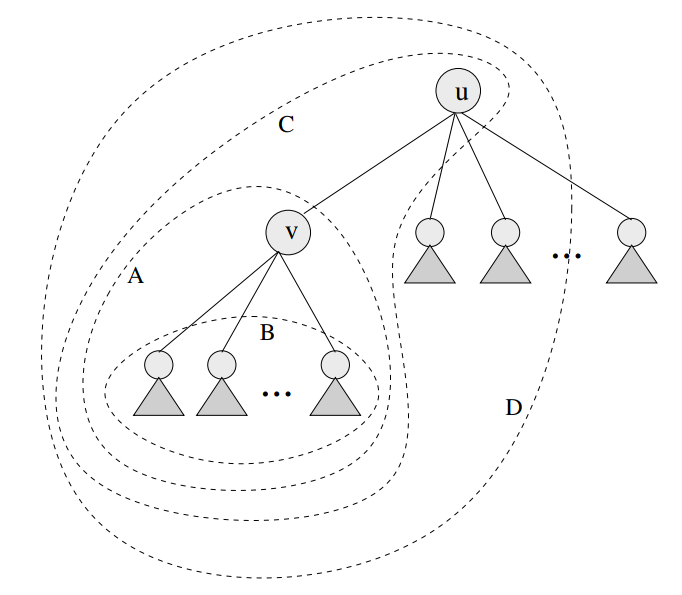
\includegraphics[width=180px]{../images/graph-cuts.png}
  \column{.4\textwidth}
  large components are refined further
  \color{red}\(s > \max\{2k-1,3k-5\}\)
  \begin{itemize}
    \item 4 distinct cut types
    \item  Steiner's Vertices\cite{aggarwal}
  \end{itemize}
  \end{columns}
\end{frame}